\documentclass[a4paper,10pt]{scrartcl}
\usepackage{babel}
\usepackage{graphicx}

\usepackage{scrlayer-scrpage}
\lohead{Aufgabe 5: Rominos}
\rohead{Team-ID: ***REMOVED***}
\cfoot*{\thepage{}}

\usepackage{listings}
\usepackage{color}
\definecolor{mygreen}{rgb}{0,0.6,0}
\definecolor{mygray}{rgb}{0.5,0.5,0.5}
\definecolor{mymauve}{rgb}{0.58,0,0.82}
\lstset{
  keywordstyle=\color{blue},
  commentstyle=\color{mygreen},
  stringstyle=\color{mymauve},
  rulecolor=\color{black},
  basicstyle=\footnotesize\ttfamily,
  numberstyle=\tiny\color{mygray},
  literate=%
  {Ö}{{\"O}}1
  {Ä}{{\"A}}1
  {Ü}{{\"U}}1
  {ß}{{\ss}}1
  {ü}{{\"u}}1
  {ä}{{\"a}}1
  {ö}{{\"o}}1
  {░}{{ }}1
  {█}{{X}}1
}

\title{Aufgabe 5: Rominos}
\author{Team-ID: ***REMOVED*** \\\\
	    Team-Name: ***REMOVED*** \\\\
	    Bearbeiter dieser Aufgabe: \\
	    ***REMOVED***\\\\}
\date{\today}

\begin{document}

\maketitle
\tableofcontents

\section{Lösungsidee}
??

\section{Umsetzung}
??

\section{Beispiele}
Hier werde ich die Beispiele aus der Aufgabe aufführen (n=4...10) und am Ende noch zwei eigene Beispiele.

\subsection{Beispiel n=4}
17 Rominos der Größe n=4 \\\\
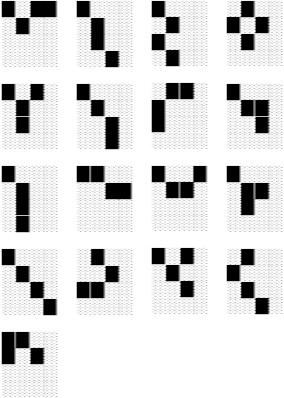
\includegraphics{4.jpg}

\subsection{Beispiel n=5}
82 Rominos der Größe n=5 \\\\
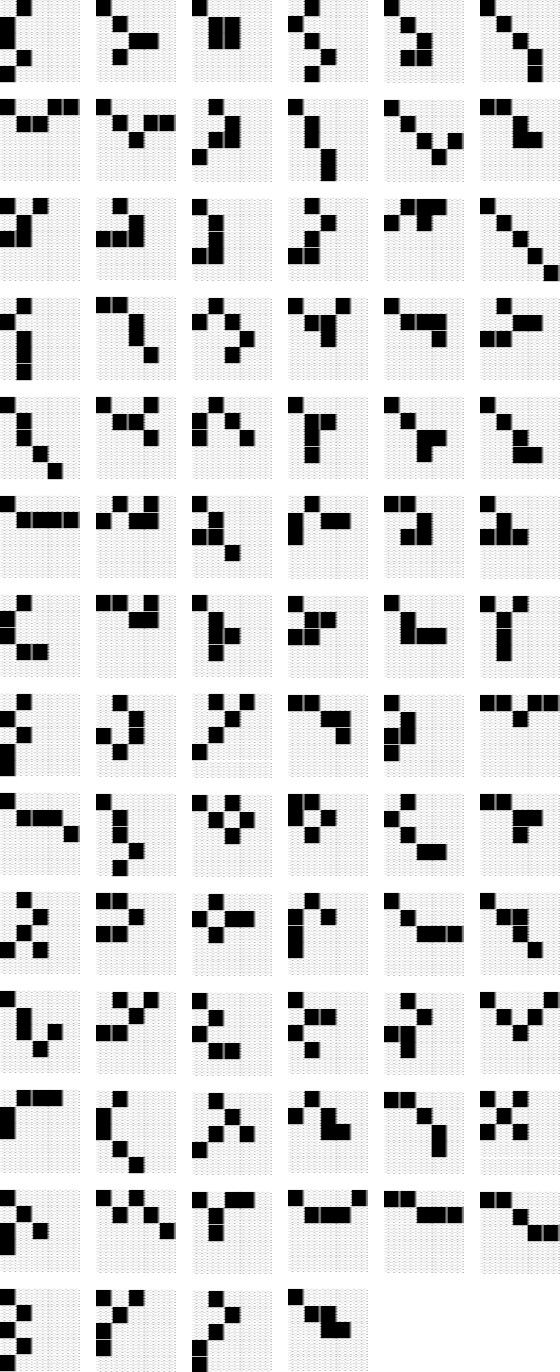
\includegraphics{5.jpg}

\subsection{Beispiel n=6}
485 Rominos der Größe n=6

\subsection{Beispiel n=7}
2892 Rominos der Größe n=6

\subsection{Beispiel n=8}
18116 Rominos der Größe n=6

\subsection{Beispiel n=9 und n=10}
Mir war es nicht möglich mit meinem Programm und meinem PC die 9er- und 10er-Rominos zu berechnen, weil ich nicht genug Arbeitsspeicher zu verfügung habe.

Bei n=9 müssten es sich um die 100 Tausend Rominos handeln und bei n=10 um die Millionen. Diese Annahme ziehe ich aus dem Verhältnis 1 zu 10 der Ergebnisse für die 7er und 8er-Rominos.

\subsection{Beispiel n=2}
Bei n=2 gibt es nur einen Romino, der auch mit meinem Programm gefunden werden kann: \\\\

\includegraphics{2.jpg}

\subsection{Beispiel n=1}
Bei n=1 gibt es keinen Romino, weil mit nur einem Quadrat keine diagonale Verbindung möglich ist.

\section{Quellcode}
\lstset{numbers=left}
\lstinputlisting[language=python]{"Aufgabe 5: Rominos/rominos.py"}

\end{document}
